\lecture{12}{15. April 2025}{Gasblandinger og fugtig luft}

\section{Gasblandinger} \label{afs:gasblanding}
I dette kapitel behandles gasblandinger, dvs. en blanding af to eller flere gasarter. Det antages i alle tilfælde at der ikke sker en kemisk reaktion mellem de indgående gasarter i gasblandingen.

Det skal understreges at der udelukkende arbejdes med gasblandinger. Der kan blot trækkes få paralleller til væskeblandinger.

\subsection{Formler for angivelse af sammensætning af en gasblanding}
For en blanding af to eller flere gasarter, hvor $n$ angiver antallet af gasarter i gasblandingen, kan følgende regler opstilles for gasblandingens samlede masse, stofmængde og volumen:
\begin{align*}
  m_{\mathrm{mix}} &= \sum_{i = 1}^{n} m_i \\
  N_{\mathrm{mix}} &= \sum_{i = 1}^{n} N_i \\
  V_{\mathrm{mix}} &= \sum_{i = 1}^{n} V_i (T_{\mathrm{mix}}, p_{\mathrm{mix}})
.\end{align*}
Forudsat at der ikke sker en kemisk reaktion gælder de første to af de ovenstående formler både for idealgasser og realgasser. Den nederste kaldes også Amagat's lov og gælder eksakt for idealgasser, men kun tilnærmet for realgasser. Derudover gælder denne kun ved fastholdt tryk og temperatur.

I mange sammenhænge kan det være hensigtsmæssigt at angive den enkelte gasarts andel af den samlede gasblanding. Her opstilles normalt formler for hhv. masseandel, molandel og volumenandel som:
\begin{align*}
  M_{a_i} &= \frac{m_i}{\sum_{i = 1}^{n} m_i} \\
  N_{a_i} &= \frac{N_i}{\sum_{i = 1}^{n} N_i} \\
  V_{a_i} &= \frac{V_i}{\sum_{i = 1}^{n} V_i}
.\end{align*}

Enheden for f.eks. masseandel er i enheden kg-gasart / kg-blanding. For en blanding af idealgasser er molandelen og volumenandelen identisk.

Desuden præsenteres her også 6 formler for omregning mellem de førnævnte andelsstørrelser:
\begin{align*}
  M_{a_i} &= \frac{N_{a_i} \cdot M_i}{\sum_{i = 1}^{n} N_{a_i} \cdot M_i} \\
  M_{a_i} &= \frac{ \frac{V_{a_i}}{R_{i,i}}}{\sum_{i = 1}^{n} \frac{V_{a_i}}{R_{i,i}}} \\
  N_{a_i} &= \frac{ \frac{M_{a_i}}{M_i}}{\sum_{i = 1}^{n} \frac{M_{a_i}}{M_{i}}} \\
  N_{a_i} &= \frac{ \frac{V_{a_i}}{R_{i,i} \cdot M_i}}{\sum_{i = 1}^{n} \frac{V_{a_i}}{R_{i,i} \cdot M_i}} \\
  V_{a_i} &= \frac{M_{a_i} \cdot R_{i,i}}{\sum_{i = 1}^{n} M_{a_i} \cdot R_{i,i}} \\
  V_{a_i} &= \frac{N_{a_i} \cdot M_i \cdot R_{i,i}}{\sum_{i = 1}^{n} N_{a_i} \cdot M_i \cdot R_{i,i}}
.\end{align*}

\subsection{Daltons lov og partialtryk}
Daltons lov udtrykker at det samlede tryk for en gasblanding $p_{\mathrm{mix}}$ er lig summen af partialtrykkene $p_i$ for de indgående gasarter:
\[ 
p_{\mathrm{mix}} = \sum_{i = 1}^{n} p_i (T_{\mathrm{mix}}, V_{\mathrm{mix}})
.\]
Denne gælder kun eksakt for idalgasser, men tilnærmet for realgasser. Endvidere er den kun gældende for fastholdt temperatur. Derudover skal alle gasarter antages at have det samme volumen til rådighed.

Partialtrykket $p_i$ for den enkelte gasart i gasblandingen defineres som:
\[ 
p_i = p_{\mathrm{mix}} \cdot \frac{N_i}{\sum_{i = 1}^{n} N_i}
.\]
Specielt for idealgasser gælder:
\[ 
p_i = p_{\mathrm{mix}} \cdot N_{a_i} = p_{\mathrm{mix}}\cdot V_{a_i}
.\]
Ønskes stofværdier eller andre karakteristike for en gasart i en gasblanding til beregninger gøres dette ud fra partialtrykket for den pågældende gasart. Eksempelvis ville man benytte partialtrykket $p_i$ i idealgasligningen til et omregne mellem stofmængde $N_i$ og volumen $V_i$. 

\subsection{Tilstandsstørrelser og stofværdier for gasblandinger}
I visse sammenhænge vil man have brug for at kende tilstandsstørrelser og stofværdier for gasblandinger. Her anføres en række formler for dette.

\subsubsection{Gaskonstant}
Gaskonstanten $R_i$ for en gasblanding kan findes som:
\begin{align*}
  R_i &= \sum_{i = 1}^{n} M_{a_i}\cdot R_{i,i} \\
  R_{i} &= \frac{1}{\sum_{i = 1}^{n} \frac{V_{a_i}}{R_{i,i}}} \\
  R_{i} &= \frac{\sum_{i = 1}^{n} N_{a_i} \cdot M_i \cdot R_{i,i}}{\sum_{i = 1}^{n} N_{a_i} \cdot M_i}
.\end{align*}

\subsubsection{Specifikt volumen}
Det specifikke volumen $v$ for en gasblanding kan findes som:
\begin{align*}
  v &= \sum_{i = 1}^{n} M_{a_i}\cdot v_i \\
  v_i &= \frac{1}{\sum_{i = 1}^{n} \frac{V_{a_i}}{v_i}} \\
  v &= \frac{\sum_{i = 1}^{n} N_{a_i} \cdot M_i \cdot v_i}{\sum_{i = 1}^{n} N_{a_i} \cdot M_i}
.\end{align*}

\subsubsection{Densitet}
Densiteten $\rho$ for en gasblanding kan findes som:
\begin{align*}
  \rho &= \frac{1}{\sum_{i = 1}^{n} \frac{M_{a_i}}{\rho_i}} \\
  \rho &= \sum_{i = 1}^{n} V_{a_i}\cdot \rho_i \\
  \rho &= \frac{\sum_{i = 1}^{n} N_{a_i} \cdot M_i}{\sum_{i = 1}^{n} \frac{N_{a_i} \cdot M_i}{\rho_i}}
.\end{align*}

\subsubsection{Molmasse}
Molmassen $M$ for en gasblanding kan findes som:
\begin{align*}
  M &= \frac{1}{\sum_{i = 1}^{n} \frac{M_{a_i}}{M_i}} \\
  M &= \frac{\sum_{i = 1}^{n} \frac{V_{a_i}}{r_{i,i}}}{\sum_{i = 1}^{n} \frac{V_{a_i}}{M_i \cdot R_{i,i}}} \\
  M &= \sum_{i = 1}^{n} N_{a_i} \cdot M_i
.\end{align*}

\subsubsection{Specifik varmekapacitet}
Den specifikke varmekapacitet, både den gældende ved en enkelt temperatur og den integrale kan findes som:
\begin{align*}
  c_v &= \sum_{i = 1}^{n} M_{a_i} \cdot c_{v,i} \\
  c_p &= \sum_{i = 1}^{n} M_{a_i} \cdot c_{p,i}
.\end{align*}
Heraf følger logisk, men betinget af at der er benyttet samme referencetemperatur for de indgående gasser at:
\begin{align*}
  u &= \sum_{i = 1}^{n} M_{a_i} \cdot u_i \\
  h &= \sum_{i = 1}^{n} M_{a_i}\cdot h_i \\
  s &= \sum_{i = 1}^{n} M_{a_i} \cdot s_i \\
.\end{align*}
Disse må under ingen omstændigheder benyttes under faseskift.

\subsubsection{Viskositet og varmeledningsevne}
Hvis en usikkerhed på 5--10\% kan accepteres kan viskositeten $\mu$ og varmeledningsevnen $\lambda$ estimeres som:
\begin{align*}
  \mu &\approx \sum_{i = 1}^{n} N_{a_i} \cdot \mu_i \\
  \lambda &\approx \sum_{i = 1}^{n} N_{a_i} \cdot \lambda_i
.\end{align*}

\subsection{Gasblandinger angivet på tør og våd basis}
I visse sammenhænge er der brug for at beregne på en gasblanding på både tør og våd basis når en af de ingående gasser er vanddamp. Angivelse af en gasblanding på tør basis indebærer blot at man sætter vandindholdet lig nul og tilpasser de resterende gassers andel således at summen af disse bliver 100\%.


\section{Fugtig luft}
På \textbf{\autoref{fig:f12_1}} ses sammensætningen af tør atmosfærisk luft.
\begin{figure} [ht]
  \centering
  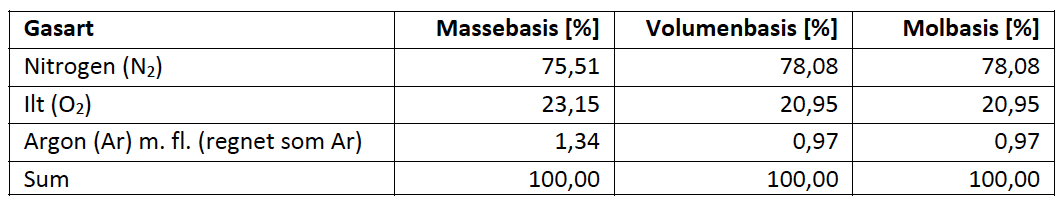
\includegraphics[width=0.75\linewidth]{./figures/f12_1.png}
  \caption{Sammensætningen af tør atmosfærisk luft}
  \label{fig:f12_1}
\end{figure}

I naturen vil atmosfærisk luft indeholde vant på dampform til en vis grad. Mængden af vanddamp er afhængig af tilstedeværelsen af vand og temperaturen. Eksempelvis finder man store mængder vand i luften i troperne og i kystnære områder. 

\subsection{Tørt og fugtigt flow af luft}
Det vil typisk være smart at dele et flow af fugtigt luft op i et flow af atmosfærisk luft og et flow af vanddamp, idet det i så fald bliver en gasblanding som er blevet behandlet i \autoref{afs:gasblanding}. Vi introducerer følgende størrelser:
\begin{align*}
  \dot{m}_{\text{våd}} &= \text{Massestrøm af den faktiske og fugtige luftmængde} \\
  \dot{m}_{\text{tør}} &= \text{Massestrøm af den tørre del af } \dot{m}_{\text{våd}} \\
  \dot{m}_{\mathrm{H}_2\mathrm{O}} &= \text{Massestrøm af den våde vanddamp}
.\end{align*}

Heraf følger følgende sammenhæng:
\[ 
\dot{m}_{\text{våd}} = \dot{m}_{\text{tør}} + \dot{m}_{\mathrm{H}_2 \mathrm{O}}
.\]
Kendes masseandelen af vanddamp i den fugtige luft kan følgende opstilles:
\begin{align*}
  \dot{m}_{\text{tør}} &= \dot{m}_{\text{våd}} \cdot (1- M_{a_{\mathrm{H}_2 \mathrm{O}}}) \\
  \dot{m}_{\mathrm{H}_2 \mathrm{O}} &= \dot{m}_{\text{våd}} - \dot{m}_{\text{tør}} = \dot{m}_{\text{våd}} \cdot M_{a_{\mathrm{H}_2 \mathrm{O}}}
.\end{align*}

\subsection{Relativ og absolut fugtighed}
Til brug i tekniske beregninger er defineret to måder at angive vandindholdet i luft. Disse er absolut vandindhold $X$ og relativt vandindhold $\varphi$. Disse er defineret som:
\begin{align*}
  X &= \frac{\text{masse af vand (damp)}}{\text{masse af tør luft}} = \frac{M_{a_{\mathrm{H}_2 \mathrm{O}}}}{1 - M_{a_{\mathrm{H}_2 \mathrm{O}}}} \\
  \varphi &= \frac{\text{Masse af vand (damp)} \cdot 100}{\text{Masse af maksimalt indhold af vand (damp)}}
.\end{align*}

Heraf fås følgende omskrivning:
\[ 
\dot{m}_{\text{våd}} = \dot{m}_{\text{tør}} + \dot{m}_{\mathrm{H}_2 \mathrm{O}} = \dot{m}_{\text{tør}} \cdot (1+X)
.\]
Det relative vandindhold $\varphi$ kan bestemmes som forholdet mellem vanddampens partialtryk for den aktuelle luft og vanddampens partialtryk ved mættet tilstand som:
\[ 
\varphi = \frac{p_{\mathrm{H}_2 \mathrm{O} } \cdot  100}{p_{\mathrm{H}_2 \mathrm{O}, \text{mæt}}}
.\]
Vandampens partialtryk ved mættet tilstand er afhængig af temperaturen og kan findes i et opslagsværk. 

\subsection{Energiindhold i fugtig luft og densitet}

\subsubsection{Entalpi baseret på vægt af den fugtige luft}
Entalpien for fugtig luft $h_{l, \text{våd}}$ kan beregnes som entalpien af tør luft $h_{l, \text{tør}}$ plus entalpien af vanddamp $h_{\mathrm{H}_2 \mathrm{O}}$ som:
\[ 
h_{l, \text{våd}} = (1 - M_{a_{\mathrm{H}_2 \mathrm{O}}}) \cdot h_{l, \text{tør}} + M_{a_{\mathrm{H}_2 \mathrm{O}}} \cdot h_{\mathrm{H}_2 \mathrm{O}}
.\]

\subsubsection{Entalpi baseret på vægt af den tørre luft andel af den fugtige luft}
Entalpi for fugtig luft $h_{l, 1+X}$ men med basis for den tørre luftandel kan beregnes som entalpi af tør luft plus entalpi af vanddamp som:
\[ 
h_{l, 1+X} = c_{p,l, \text{tør}}(p,T) \cdot T + X \cdot \left[ c_{p, \mathrm{damp}}(p,T) \cdot T + r_0 \right]
.\]

\subsubsection{Densitet for fugtig luft som funktion af den absolutte fugtighed}
Kendes den absolutte fugtighed $X$ kan densitet for den fugtige luft ved normaltilstanden bestemmes af:
\[ 
\rho_{(\qty{0}{\celsius}, \qty{101325}{Pa}, X)} = \rho_{(\qty{0}{\celsius}, \qty{101325}{Pa},\text{tør})} \cdot \frac{1+x}{1+\num{1,609} \cdot X}
.\]

Ønskes densiteten bestemt ved en anden tilstand, f.eks. \qty{10}{\celsius} og \qty{200}{Pa} kan benyttes:
\[ 
\rho_{(\qty{10}{\celsius}, \qty{200}{Pa} )} = \rho_{(\qty{0}{\celsius}, \qty{101325}{Pa}, X)} \cdot \frac{273}{273+10} \cdot \frac{200}{\num{101325} }
.\]

\subsection{Masse- og energibevarelse i knudepunkter}
Formlerne på \textbf{\autoref{fig:f11_4}} kan opstilles for masse- og energibevarelse for fugtig luft i knudepunkter. 

\begin{figure} [ht]
  \centering
  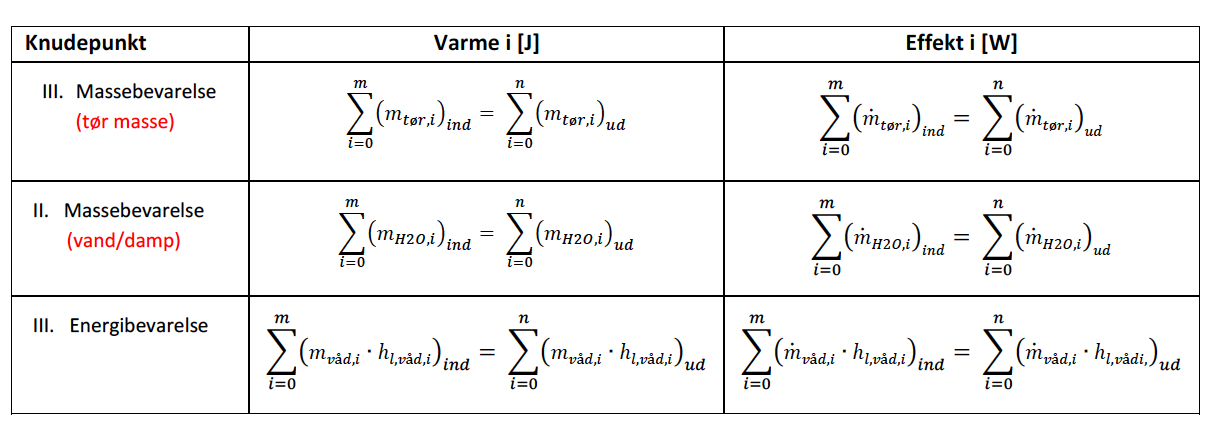
\includegraphics[width=0.5\linewidth]{./figures/f11_4.png}
  \caption{Formler til knudepunktsberegninger på fugtig luft}
  \label{fig:f11_4}
\end{figure}

De tre formler under f.eks. ``effekt'' i \textbf{\autoref{fig:f11_4}} giver mulighed for at bestemme tre ubekendte.


\subsection{Molliere diagram}
Det er generelt meget omfangsrigt at foretage beregninger på fugtig luft. Nogle af beregningerne kan lettes vha. et diagram benævnt et ``Molliere diagram`' eller et ``$T$-$X$ diagram'' dvs. med temperatyren $T$ på $y$-aksen og den absolutte fugtighed $X$ på $x$-aksen same kurve for entalpi og relativ fugtighed. Derudover kan mætningstrykket for en given temperatur aflæses. Det skal fremhæves at et Molliere diagram er lavet for et bestemt tryk. Ændres trykket skal et nyt diagram fremstilles.

I visse sammenhænge ser man også Molliere diagrammer lavet som et $h$-$x$ diagram. 

\begin{figure} [ht]
  \centering
  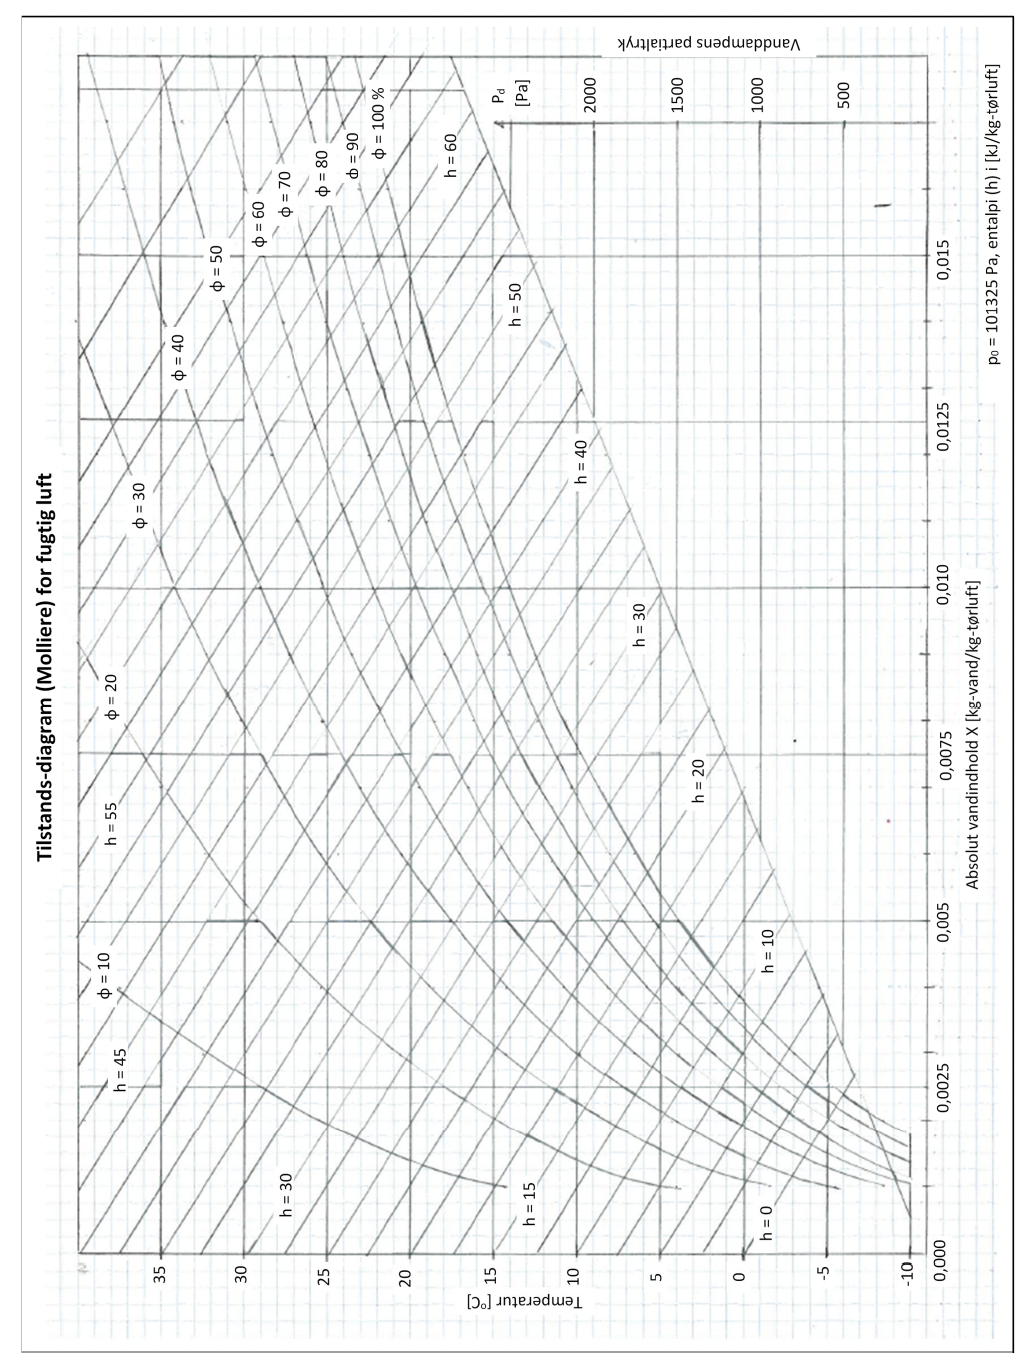
\includegraphics[width=0.5\linewidth, angle=-90]{./figures/f11_5.png}
  \caption{Eksempel på Molliere diagram for atmosfæretrykket $p = \qty{101325}{Pa}$}
  \label{fig:f11_5}
\end{figure}

For mere information om konstruktion og aflæsning af Molliere diagrammer se den fremragende vejledning på s. 244 \& 247 i bogen (s. 245 \% 248 i PDF'en). 

\subsection{Opvarmning og afkøling af fugtig luft – sensibel energiændring alene}
Når et flow af fugtig luft opvarmes eller afkøles kan det betrages som en procesændring for et åbent system, hvor der hhv. tilføres og afgives en varmeeffekt. Da trykket er konstant er det en isobarisk proces. Derfor kan følgende formel benyttes:
\[ 
\dot{Q} = \dot{m} \cdot (h_2 - h_1) = \dot{m} \cdot c_{p,m} \cdot \left( T_2 - T_1 \right)
.\]
Der er her indsat en middelværdi for det specifikke varmefylde for det generelle tilfælde, hvor den specifikke varmefylde ikke antages at være konstant. 

Under forudsætning af at der ikke sker et faseskift af vanddampen i den fugtige luft, dvs. kondensering til flydende vand, vil der ved en opvarmning eller en afkøling af et flow af fugtigt luft være én parameter, som forbliver konstant, og det er den absolutte fugtighed $X$. Dette betyder, at processforløbet ved en opvarmning eller en afkøling af et flow af fugtigt luft er en vertikal linje i $T$-$X$ diagrammet på Molliere diagrammer som \textbf{\autoref{fig:f11_5}}. Da der ikke sker et faseskift for vanddampen vil der alene være tale om en ændring af temperaturen proportionalt med tilførsel eller fjernelse af energi.

Under samme forudsætning, og ved en opvarmning eller afkøling af et flow af fugtigt luft vil masseandel af vanddamp i den fugtige luftstrøm $M_{a_{\mathrm{H}_2 \mathrm{O}}}$ og partialtrykket for vanddampen $p_{\mathrm{H}_2 \mathrm{O}}$ ligeledes være konstante.

Vi har generelt også følgende formel for den nødvendige effekt ved en temperaturændring af et flow af fugtigt luft:
\begin{multline*}
  \dot{Q} = \dot{m}_{l, \text{våd}} \cdot \big( \left( 1 - M_{a_{\mathrm{H}_2 \mathrm{O}}} \right) \cdot \left( c_{p, l, \text{tør}, 2} \left( p_2, T_2 \right) \cdot T_2 - c_{p, l, \text{tør}, 1} \left( p_1, T_1 \right) \cdot T_1 \right) \\
  + M_{a_{\mathrm{H}_2 \mathrm{O}}} \cdot \left( h \left( p_{\mathrm{H}_2 \mathrm{O}}, T_2 \right) - h \left( p_{\mathrm{H}_2 \mathrm{O}}, T_1 \right) \right) \big)
.\end{multline*}
Man burde egentligt benytte den integrale specifikke varmekapacitet $c_{p, \text{int}}$ i stedet for den specifikke varmekapacitet $c_p$ men er man tæt på referencepunktet for beregning af entalpi ($T = \qty{0}{\celsius} $) er forskellen ikke stor. 

Vi har også formlen:
\begin{align*}
  \dot{Q} &= \dot{m}_{t, \text{tør}} \cdot \left( h_{l,1 + X,2} - h_{l,1 + X,1} \right) \\
          &= \dot{m}_{l ,\text{tør}} \cdot \left( \num{1,006} + X \cdot \num{1,86}  \right) \cdot \left( T_2 - T_1 \right)
.\end{align*}


\subsection{Beffugtning og affugtning af fugtig luft}

\subsubsection{Affugtning af fugtig luft}
Generelt affugter man enten fugtig luft kemisk vha. adsorption eller ved afkøling.

Affugtning ved adsoprtion sker ved at bringe den fugtige luft i kontakt med f.eks. calciumklorid eller silica gel. Disse stoffer er hygroskopiske, dvs. de tiltrækker og optager vand indtil en vis grænse ved en given temperatur. Processen kan reverseres ved at opvarme materialet hvorved det vil afgive vandet igen. Dette kendes fra de små hvide poser i bl.a. skotøjsæsker.

Affugtning kan også ske ved afkøling af den fugtige luftstrøm. Antag eksempelvis at man på Molliere diagrammet på \textbf{\autoref{fig:f11_5}} forsøger at køle ned til et punkt under $\phi = 100\%$-kurven. Man kan ikke køle igennem denne kurve da vanddamp i så fald begynder at kondensere. Derfor vil man langsomt bevæge sig langs $\phi=100\%$-kurven videre nedad, hvis nedkølingen fortsættes.

\subsubsection{Beffugtning af fugtig luft}
Befugtning kan ske på flere måder, herunder:
\begin{itemize}
  \item Direkte blanding/mixning af en luftstrøm med recirckuleret vand
  \item Fortøvning af koldt eller varmt vand via dyser direkte i luftstrømmen
  \item Injektion af damp via dyser direkte i luftstrømmen
\end{itemize}
Her behandles udelukkende pkt. 1, dvs. direkte blanding af en luftstrøm med recirkuleret vand. Dette er vist i procesdiagramet på \textbf{\autoref{fig:f12_3}}. Foruden at opnå en befugtning af luften vil der også ske en afkøling således, at temperaturen falder for den behandlede luftstrøm. Dette er behandlet nærmere i \textbf{\autoref{afs:term}}.

\begin{figure} [ht]
  \centering
  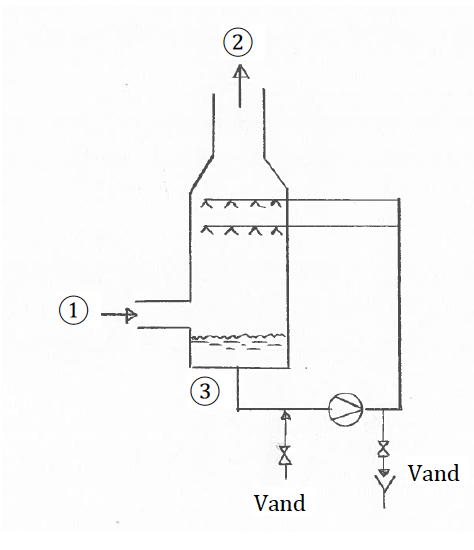
\includegraphics[width=0.5\linewidth]{./figures/f12_3.png}
  \caption{Procesdiagram for befugtning af luft ved direkte blanding med recirkuleret vand}
  \label{fig:f12_3}
\end{figure}

For at kompensere for forbrugt vand i processen må der spædes nyt vand til. Det fordampede vand vil være rent, og eventuelle salte og mineraler i det tilspædte vand vil blive ophobet i det recirkulerede vand. Derfor må man aflede en vis mængde vand til kloakken for at opretholde en maksimal saltkoncentration i det recirkulerede vand. Efter processen (pkt. 2) installeres et dråbefang der sørger for at ingen vanddråber fortsætter med luftstrømmen rundt.

\subsection{Tørt og vådt termometer} \label{afs:term}
To ens termometre i den samme luftstrøm vil vise forskellige resultater, hvis den ene er pakket ind i vådt vat og den anden ikke er. Dette skyldes at for termometeret pakket ind i vat, vil vandet fordampe isentalpisk og derved afkøle vattet.

Det tørre termometer viser omgivelsestemperaturen og det våde termometer vil vise en lavere temperatur end omgivelsestemperaturen.
